\documentclass[11pt]{article}
\usepackage[margin=1in]{geometry}
\usepackage{graphicx}
\usepackage{booktabs}
\usepackage{amsmath}
\usepackage{hyperref}
\usepackage{xcolor}
\hypersetup{colorlinks=true, urlcolor=blue, linkcolor=black, citecolor=black}
\graphicspath{{../experiments/v0/figures/}}

\title{Redox Networks: A Conservation-Based Equilibrium Neural Network,\\
and Why Diffusion-Style Models Are Capped on Tabular Data}
\author{ALMoatsim\\
Independent Researcher\\
\texttt{moutasem.hamdi14@gmail.com}\\
ORCID: \href{https://orcid.org/0009-0002-6350-1534}{0009-0002-6350-1534}}
\date{}

\begin{document}
\maketitle

\begin{abstract}
We introduce the Redox Network, a neural network whose units do not freely produce outputs.
Instead, each unit holds an amount of a conserved quantity that we call charge, and units
pass charge to one another along learned connections until the system reaches a balance (an
equilibrium). The design is inspired by reduction-oxidation (redox) chemistry, where atoms
donate and accept electrons and a reaction settles at a stable state. We add two further
ingredients: a soft preference for charge to rest at discrete levels, and a hard, learned
gate on each input feature that lets the network ignore a feature entirely.

We study the model on tabular data, the setting where gradient-boosted decision trees
(GBDTs) such as XGBoost still beat neural networks. Our model has one clear strength: with
the hard feature gate it becomes robust to useless (uninformative) features. When we add 100
pure-noise columns to a dataset, our model's accuracy drops by less than half a point, the
smallest drop of every model we tested, including XGBoost and LightGBM. The standard neural
networks fall far more (a multi-layer perceptron by about 9 points, a tabular ResNet by
about 12, TabNet by 6, FT-Transformer by 3), so at high noise our model becomes the most
accurate neural network of all of them. We get this at a small price: on perfectly clean
data our model is about 1 to 2 points behind the others. This kind of robustness to useless
features is a property that standard neural networks lack.

Our model does not, however, beat gradient-boosted trees on clean accuracy. We give a simple
explanation, supported by both existing theory and our own experiments. Reaching an
equilibrium is, in mathematical terms, a smoothing (low-pass) operation: it averages
neighbouring values together. Tabular target functions are usually jagged, not smooth, and
the known reason neural networks struggle on tabular data is exactly a bias toward smooth
functions. So our central mechanism works against the structure of the data. We confirm this
directly: when we feed the model sharp, tree-like features, the equilibrium step blurs them
and accuracy drops relative to a plain linear readout on the same features. We conclude that
conservation-and-equilibrium models are a poor fit for tabular accuracy, but a natural fit
for problems whose targets are genuinely smooth or governed by conservation laws (for
example physical fields and graphs).
\end{abstract}

\section{Introduction}

Most neural networks compute in one direction. An input enters, passes through a stack of
layers, and an output comes out the other end. Each unit is free to produce any value it
likes from its inputs. Nothing is conserved along the way.

We take a different starting point, borrowed from chemistry. In a reduction-oxidation (redox)
reaction, some atoms give up electrons (they are oxidised) and others take them up (they are
reduced). Electrons are not created or destroyed; they move from donor to acceptor, and the
reaction settles at a stable, low-energy state. We asked a simple question: what happens if a
neural network works the same way? Units hold a conserved quantity, pass it to one another,
and the answer is read off the state the system settles into, rather than computed in a
single forward sweep.

We call the result a Redox Network. The contribution of this paper is threefold. First, we
define the model: a layered network in which a fixed budget of a conserved charge flows
between units along learned connections and relaxes to an equilibrium, with two extra design
choices, a soft preference for discrete charge levels and a hard, learned per-feature gate.
Second, we show the model has a property that ordinary neural networks famously lack:
robustness to uninformative features, the headline strength of decision trees. Third, and
most useful for future work, we explain a limitation honestly and precisely: the model does
not beat gradient-boosted trees on clean tabular accuracy, and we show this is not a tuning
problem but a consequence of the mathematics. We chose tabular data on purpose: it is the one
common domain where neural networks still lose to a simpler method, so it is a clean test of
whether a new mechanism brings anything.

\section{Background and related work}

\textbf{Why trees beat neural networks on tabular data.} Grinsztajn et al.~\cite{grinsztajn}
give two reasons. The first is rotation invariance. A multi-layer perceptron trained by
gradient descent is a rotationally invariant learner in the sense of Ng~\cite{ng}; if you
rotate the feature axes, its behaviour does not change. But a rotation mixes the columns
together, and in a table the columns (``age'', ``income'') are meaningful on their own. Trees
split on one column at a time, so they are not rotation invariant and they exploit this
structure. Ng~\cite{ng} proves that any rotationally invariant learner needs a number of
samples that grows at least linearly with the number of irrelevant features, against only
logarithmic growth for axis-aware methods (Figure~\ref{fig:rotation}).

\begin{figure}[t]\centering
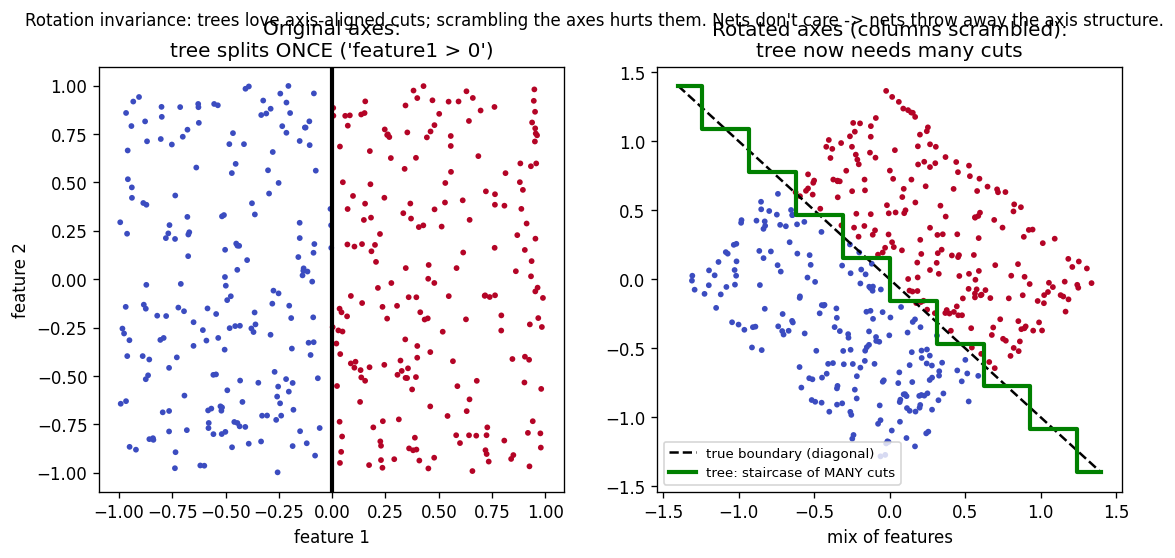
\includegraphics[width=0.92\linewidth]{rotation.png}
\caption{Rotation invariance. Left: the classes split along a single feature, so a tree needs
one axis-aligned cut. Right: after the feature axes are rotated (the columns are mixed
together), the same boundary needs a staircase of many cuts. A neural network is blind to
this difference, so it cannot use the meaningful per-column structure that trees rely on.}
\label{fig:rotation}
\end{figure}

The second reason is smoothness. Gradient-descent-trained networks are biased toward
low-frequency (smooth) functions~\cite{rahaman}; tabular targets are often jagged and
piecewise constant, which trees fit easily and smooth models do not.

\textbf{Trees as a kernel.} A decision forest can be read as a learned similarity: two points
are similar if they fall in the same leaf~\cite{biau}. This leaf co-occurrence kernel is
axis-aligned, non-smooth, and adapted to the data. An infinite ensemble of axis-aligned
random partitions (the Mondrian kernel~\cite{balog}) converges to the L1 Laplace kernel,
which sits at the same non-smooth-admitting end of the spectrum as the neural tangent kernel
of a ReLU network~\cite{geifman,chen}. This view motivated our final experiment.

\textbf{Equilibrium and energy-based models.} Networks that settle to a fixed point have a
long history: Hopfield networks, energy-based models, Equilibrium Propagation~\cite{scellier},
and Deep Equilibrium Models~\cite{bai}. Our model is in this family. The new parts are the
conservation law (charge is neither created nor destroyed inside the network) and the
redox-style donor/acceptor transfer.

\textbf{Differentiable feature selection.} Our hard gate uses the L0 / Hard-Concrete
relaxation of Louizos et al.~\cite{louizos}, with a straight-through estimator so a
switched-off feature is exactly zero in the forward pass while gradients still flow.

\textbf{Neural networks for tabular data.} Many neural designs target this setting, including
NODE~\cite{node}, TabNet, and FT-Transformer. NODE is the most relevant to us: it builds
differentiable, axis-aligned decision trees, which is close to the feature map we use in our
final experiment.

\section{The Redox Network}

\subsection{Units, charge, and conservation}
The network has units arranged in layers (input, one or more hidden, output). Each unit $i$
holds a real-valued charge $q_i$. A fixed total budget $Q=\sum_i q_i$ is poured in and the
total never changes during settling; charge only moves between units. This is the
conservation law, and it is the core of the design. Each unit has a learned greed $\chi_i$
(how strongly it pulls charge toward itself). Adjacent layers are joined by learned weights
$W$ (the connections, or pipes). See Figure~\ref{fig:arch}.

\begin{figure}[t]\centering
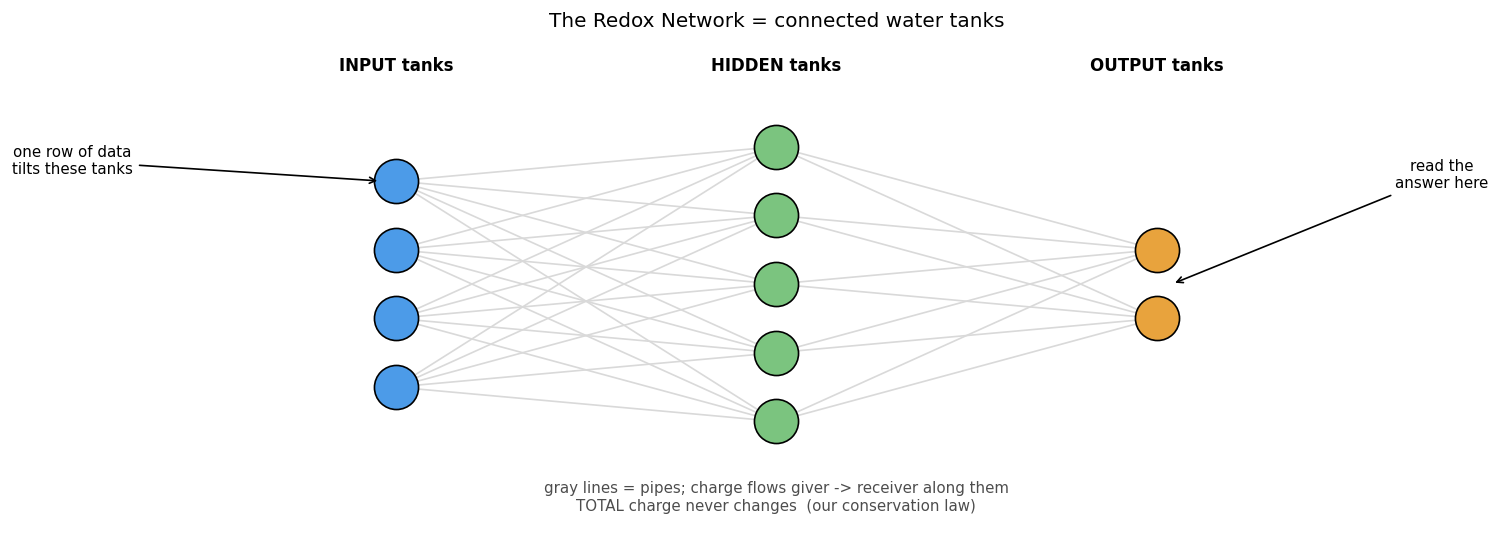
\includegraphics[width=0.78\linewidth]{architecture.png}
\caption{The Redox Network as connected tanks joined by pipes. A fixed amount of charge is
poured in, flows between units along the connections, and settles to a balance. The
prediction is read from the settled state. The total charge never changes.}
\label{fig:arch}
\end{figure}

\subsection{Energy and the settling dynamics}
We define a single energy for a configuration of charges, subject to $\sum_i q_i = Q$:
\begin{equation}
E(q) = \sum_i \Big(\tfrac{1}{2} q_i^2 - \chi_i q_i\Big)
     - \sum_{i \in \text{input}} h_i(x)\, q_i
     - \sum_{(i,j) \in E} W_{ij}\, q_i q_j
     + \beta \sum_i v(q_i).
\end{equation}
Here $h(x)$ is the input after a learned intake map, and $v(q) = 1 - \cos(2\pi q)$ is a gentle
washboard with minima at integers, so charge prefers to rest near whole numbers (a soft
version of discrete oxidation states). The strength $\beta$ can be increased during training
to sharpen the levels. The per-unit potential is $\mu_i = \partial E / \partial q_i$. Settling
moves charge from high-potential to low-potential units along each edge, which lowers $E$
while keeping the total fixed:
\begin{equation}
\text{flow}_{ij} = \eta\, W_{ij}\,(\mu_i - \mu_j), \qquad
q_i \leftarrow q_i - \!\sum_j \text{flow}_{ij}, \quad
q_j \leftarrow q_j + \!\sum_j \text{flow}_{ij}.
\end{equation}
We repeat for $T$ steps. The self-limiting term $\tfrac{1}{2} q_i^2$ raises a unit's potential
as it fills, so flow dies out and the system reaches a balance instead of collapsing into one
unit (Figure~\ref{fig:settle}). We bound the connection strengths so this iteration is stable.

\begin{figure}[t]\centering
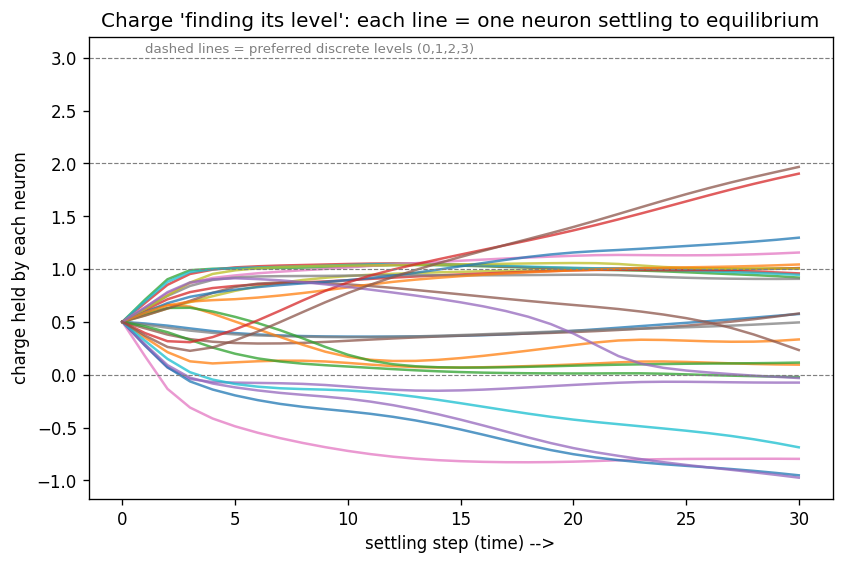
\includegraphics[width=0.8\linewidth]{settling.png}
\caption{Charge settling to equilibrium for one input. Each line is one unit's charge over the
settling steps. The values start equal, redistribute, and come to rest near the preferred
discrete levels (dashed lines).}
\label{fig:settle}
\end{figure}

The prediction is read from the settled charges of the output units through a small linear
layer. We train by unrolling the $T$ settling steps and back-propagating an ordinary task loss
(cross-entropy), plus a small penalty that rewards reaching a settled state.

\subsection{The hard feature gate}
To let the network ignore a feature, we put a gate $g_j \in \{0,1\}$ on each input feature $j$,
so the intake sees $g_j x_j$. We parameterise $g_j$ with the Hard-Concrete
distribution~\cite{louizos} and a straight-through estimator: in the forward pass the gate is
exactly 0 or 1, so a closed gate removes the feature completely (the later layers cannot leak
it back by growing their weights). We add a penalty on the number of open gates and train in
two stages: first the gates with the rest of the intake held simple, then the full model.

\section{Experiments}

\subsection{Setup}
We use numerical-feature binary-classification datasets from the tabular benchmark of
Grinsztajn et al.~\cite{grinsztajn}, specifically MagicTelescope and electricity, with up to
8{,}000 training rows, standardised features, fixed splits, and results averaged over multiple
seeds. Baselines are two gradient-boosted tree libraries (XGBoost, LightGBM) and four neural
networks: a tuned MLP, a tabular ResNet, an FT-Transformer, and TabNet. We report test
accuracy. We verified that total charge stays constant during settling and the per-step flow
shrinks toward zero, so the network really does reach an equilibrium.

\subsection{Robustness to uninformative features}
We add $k$ columns of pure Gaussian noise and measure accuracy at $k=0$ and $k=100$.

\begin{table}[h]\centering
\begin{tabular}{lccc}
\toprule
Model & clean ($k{=}0$) & $k{=}100$ & accuracy lost \\
\midrule
XGBoost & 0.885 & 0.868 & 1.7 \\
LightGBM & 0.884 & 0.869 & 1.5 \\
MLP & 0.877 & 0.789 & 8.8 \\
ResNet & 0.882 & 0.762 & 11.9 \\
FT-Transformer & 0.878 & 0.851 & 2.7 \\
TabNet & 0.868 & 0.804 & 6.4 \\
\textbf{Redox (ours)} & 0.864 & 0.860 & \textbf{0.5} \\
\bottomrule
\end{tabular}
\caption{MagicTelescope.}
\end{table}

\begin{table}[h]\centering
\begin{tabular}{lccc}
\toprule
Model & clean ($k{=}0$) & $k{=}100$ & accuracy lost \\
\midrule
XGBoost & 0.843 & 0.811 & 3.2 \\
LightGBM & 0.842 & 0.808 & 3.4 \\
MLP & 0.783 & 0.732 & 5.1 \\
ResNet & 0.797 & 0.675 & 12.2 \\
FT-Transformer & 0.795 & 0.730 & 6.4 \\
\textbf{Redox (ours)} & 0.775 & 0.772 & \textbf{0.3} \\
\bottomrule
\end{tabular}
\caption{electricity.}
\end{table}

On both datasets our model loses the least accuracy of any model as noise is added, less even
than the gradient-boosted trees, so at 100 noise columns it is the most accurate neural
network, ahead of the MLP, ResNet, FT-Transformer, and TabNet (Figure~\ref{fig:robust}). This
is our main positive result: with a hard feature gate, a neural network reaches (and on these
two datasets slightly exceeds) the tree-style immunity to useless features that ordinary
neural networks lack. The cost is small: on fully clean data the hard gate trims a few weak
but useful features, which is why our clean accuracy sits about 1 to 2 points below the other
models; a lower gate penalty recovers part of this while keeping the flat behaviour.

\begin{figure}[t]\centering
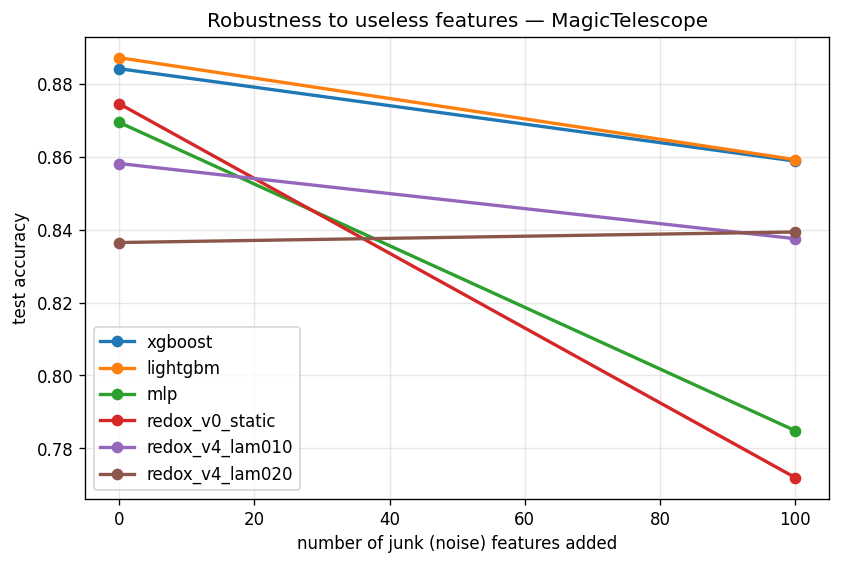
\includegraphics[width=0.7\linewidth]{robustness_MagicTelescope.png}
\caption{Test accuracy as junk (noise) features are added, on MagicTelescope. The Redox
Network (ours) stays nearly flat, while the standard neural networks fall sharply; the trees
are also robust.}
\label{fig:robust}
\end{figure}

\subsection{Clean accuracy, and an honest negative result}
On clean data our model is competitive with the MLP but below the trees. To test whether the
gap is about the input representation, we built a version with a tree-like front end: a small
set of learned, axis-aligned soft decision trees turns each row into leaf-membership features,
fed either to a plain linear layer or to our settling dynamics.

\begin{table}[h]\centering
\begin{tabular}{lcc}
\toprule
Model & MagicTelescope & electricity \\
\midrule
XGBoost & 0.885 & 0.843 \\
Tree features + linear readout & 0.880 & 0.792 \\
Tree features + our settling & 0.875 & 0.778 \\
\bottomrule
\end{tabular}
\caption{The axis-aligned feature map alone nearly matches XGBoost; adding our settling makes
it worse.}
\end{table}

The axis-aligned feature map alone closes most of the gap to XGBoost on MagicTelescope (0.880
vs 0.885), which confirms the representation matters. But adding our settling dynamics on top
makes accuracy worse, not better, on both datasets.

\subsection{Why settling hurts: a smoothing analysis}
This is not a tuning artefact; it follows from what equilibrium does. Settling a conserved
quantity over a graph until it balances is a diffusion process, and diffusion is a low-pass
filter: it averages neighbouring values and rounds off sharp changes. Tabular targets are
jagged, and the established reason neural networks lose on tabular data is a bias toward smooth
functions~\cite{grinsztajn,rahaman}. So our central mechanism applies a smoother to a problem
whose difficulty is precisely its lack of smoothness (Figure~\ref{fig:smooth}). When we hand
the settling step the sharp leaf features, it blurs them and the prediction worsens. This also
explains why our only clear win comes from the hard gate and not from the settling: feature
selection and smoothing are different operations, and only the former helps here.

\begin{figure}[t]\centering
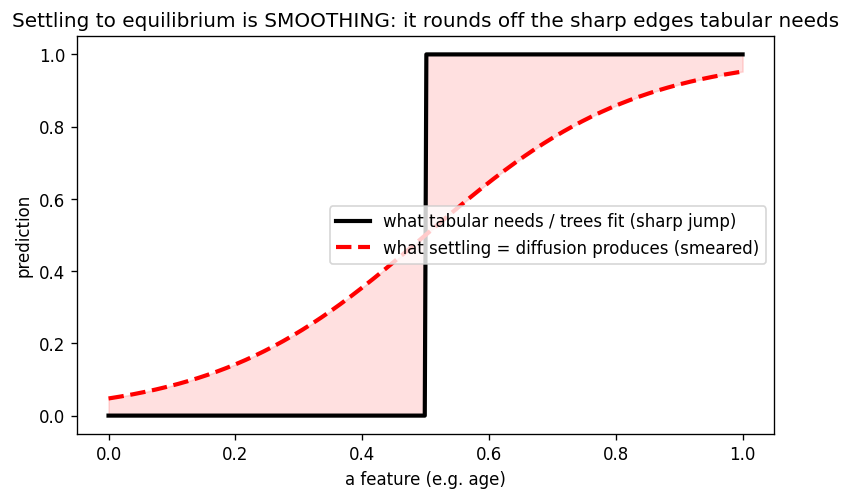
\includegraphics[width=0.7\linewidth]{smoothing.png}
\caption{Settling is smoothing. The sharp step is what tabular targets need, and what trees
fit; the rounded curve is what a diffusion / equilibrium step produces, blurring the edge.}
\label{fig:smooth}
\end{figure}

\section{Discussion}
The Redox Network is a working, novel mechanism with one genuine strength on tabular data,
tree-like robustness to useless features, and one clear limitation that we now understand. The
limitation is structural: equilibrium and diffusion are smoothing operations, and tabular
accuracy rewards sharpness. No amount of tuning changes this, because it is a property of the
mathematics. This points somewhere useful: a mechanism that smooths and conserves should do
well where the target really is smooth, or where a conservation law is part of the problem,
such as physical fields, diffusion and heat-like processes, and data on graphs (where settling
is exactly the kind of message passing that graph networks already use).

\section{Limitations}
Our experiments cover two datasets; a fuller study would use the complete benchmark
of~\cite{grinsztajn} and add further methods such as NODE and TabPFN. The robustness gate uses
a known relaxation~\cite{louizos}; the contribution is its use inside this architecture, not
the gate itself. The smoothing argument is supported by existing theory and by our ablation,
but we state it as an explanation rather than a formal theorem; a precise statement of settling
as a graph low-pass filter is left for future work. Finally, settling is sequential and adds
compute over a single forward pass.

\section{Conclusion}
We presented the Redox Network, a neural network built on a conservation law and an
equilibrium, inspired by redox chemistry. It earns a real property that ordinary networks
lack, robustness to uninformative features, and we showed, with theory and experiment, why its
core mechanism cannot win on clean tabular accuracy: settling is smoothing, and tabular data is
not smooth. The honest mapping of where this mechanism helps and where it cannot is the most
useful thing the paper offers.

\paragraph{Reproducibility.} All code, model definitions, experiment scripts, and figures are
available at \url{https://github.com/Al-Mo3tasem/redox-networks}.

\begin{thebibliography}{99}
\bibitem{grinsztajn} L. Grinsztajn, E. Oyallon, G. Varoquaux. Why do tree-based models still outperform deep learning on typical tabular data? NeurIPS 2022 (arXiv:2207.08815).
\bibitem{ng} A. Y. Ng. Feature selection, L1 vs. L2 regularization, and rotational invariance. ICML 2004.
\bibitem{rahaman} N. Rahaman et al. On the spectral bias of neural networks. ICML 2019.
\bibitem{biau} G. Biau, E. Scornet. A random forest guided tour. TEST 25, 2016 (arXiv:1511.05741).
\bibitem{balog} M. Balog, B. Lakshminarayanan, Z. Ghahramani, D. Roy, Y. W. Teh. The Mondrian kernel. UAI 2016 (arXiv:1606.05241).
\bibitem{geifman} A. Geifman et al. On the similarity between the Laplace and neural tangent kernels. NeurIPS 2020.
\bibitem{chen} L. Chen, S. Xu. Deep neural tangent kernel and Laplace kernel have the same RKHS. ICLR 2021 (arXiv:2009.10683).
\bibitem{scellier} B. Scellier, Y. Bengio. Equilibrium propagation. Frontiers in Computational Neuroscience, 2017.
\bibitem{bai} S. Bai, J. Z. Kolter, V. Koltun. Deep equilibrium models. NeurIPS 2019.
\bibitem{louizos} C. Louizos, M. Welling, D. P. Kingma. Learning sparse neural networks through L0 regularization. ICLR 2018.
\bibitem{node} S. Popov, S. Morozov, A. Babenko. Neural oblivious decision ensembles for deep learning on tabular data. ICLR 2020 (arXiv:1909.06312).
\bibitem{xgboost} T. Chen, C. Guestrin. XGBoost: a scalable tree boosting system. KDD 2016.
\end{thebibliography}

\end{document}
